\documentclass[english, a4paper]{article}

\usepackage[T1]{fontenc}    % Riktig fontencoding
\usepackage[utf8]{inputenc} % Riktig tegnsett
\usepackage{babel}          % Ordelingsregler, osv
\usepackage{graphicx}       % Inkludere bilder
\usepackage{booktabs}       % Ordentlige tabeller
\usepackage{url}            % Skrive url-er
\usepackage{textcomp}       % Den greske bokstaven micro i text-mode
\usepackage{units}          % Skrive enheter riktig
\usepackage{float}          % Figurer dukker opp der du ber om
\usepackage{lipsum}         % Blindtekst
\usepackage{subcaption} 
\usepackage{color}
\usepackage{amsmath}  
\usepackage{hyperref}
\usepackage{pagecolor}
%\usepackage{minted}
\usepackage{braket} 
\usepackage{multicol}
\usepackage{listings}    %Add source code
\usepackage{amsfonts}
\usepackage{setspace}
\usepackage[cm]{fullpage}		% Smalere marger.
\usepackage{verbatim} % kommentarfelt.
\usepackage{tabularx}
\usepackage{booktabs}
\usepackage{tikz}				

\usetikzlibrary{shapes,arrows}	
\usetikzlibrary{arrows,decorations.markings}

\definecolor{decisionColor}{HTML}{DEE1B2}
\definecolor{nodeColor}{HTML}{B2DFE2}

\tikzstyle{roundrect}=[rectangle, rounded corners, minimum width=3cm, minimum height=1cm, text centered, draw=black, fill=nodeColor, text width=3.5cm] 
\tikzstyle{decision} = [diamond, minimum width=3.7cm, minimum height=3.2cm, text centered, draw=black, fill=decisionColor, scale=1, text width=2.05cm]
\tikzstyle{arrow} = [decoration={markings,mark=at position 1 with
	{\arrow[scale=1.5,>=stealth]{>}}},postaction={decorate}]

\setlength{\columnseprule}{1pt}	%(width of separationline)
\setlength{\columnsep}{1.0cm}	%(space from separation line)
\newcommand\lr[1]{\left(#1\right)} 
\newcommand\bk[1]{\langle#1\rangle} 
\newcommand\uu[1]{\underline{\underline{#1}}} % Understreker dobbelt.
\newcolumntype{Y}{>{\centering\arraybackslash}X}
\definecolor{qc}{rgb}{0,0.4,0}
\definecolor{LightBlue}{rgb}{0.8, 0.8, 0.9}
\hypersetup{
	colorlinks,
	linkcolor={red!30!black},
	citecolor={blue!50!black},
	urlcolor={blue!80!black}
}
% JF i margen
\makeatletter
\renewcommand{\subsubsection}{\@startsection{subsubsection}{3}{0pt}%
	{-\baselineskip}{0.5\baselineskip}{\bf\large}}
\makeatother
\newcommand{\jf}[1]{\subsubsection*{JF #1}\vspace*{-2\baselineskip}}

\newcommand{\bm}[1]{\mathbf{#1}}

% Skru av seksjonsnummerering (-1)
\setcounter{secnumdepth}{3}

\begin{document}
	%\pagecolor{black!50!}
	\renewcommand{\figurename}{Figure}
	% Forside
	\begin{titlepage}
		\begin{center}
			
			\textsc{\Large FYS4411 - Computational quantum mechanics }\\[0.5cm]
			\textsc{\Large Spring 2016}\\[1.5cm]
			\rule{\linewidth}{0.5mm} \\[0.4cm]
			{ \huge \bfseries  Project 2;\\ Variational Monte Carlo studies of electronic systems}\\[0.10cm]
			\rule{\linewidth}{0.5mm} \\[1.5cm]
			
			{\Large Github repository:} \\*[0.4cm]
			\url{https://github.com/filiphl/FYS4411.git}
			
			\vspace{13.5cm}
			
			% Av hvem?
			\begin{minipage}{\textwidth}
				\begin{minipage}{0.49\textwidth}
					\begin{center} \large
						Sean Bruce Sangolt Miller\\
						{\footnotesize s.b.s.miller@fys.uio.no}
					\end{center}
				\end{minipage}
				\quad
				\begin{minipage}{0.49\textwidth}
					\begin{center} \large
						Filip Henrik Larsen\\
						{\footnotesize filiphenriklarsen@gmail.com}
					\end{center}
				\end{minipage}
			\end{minipage}
			\vfill
			
			% Dato nederst
			\large{Date: \today}
			
		\end{center}
	\end{titlepage}
	%%%%%%%%%%%%%%%%%%%%%%%%%%%%%%%%%%%
	
	\begin{abstract}
		
	\end{abstract}
	
	
	%%%%%%%%%%%%%%%%%%%%%%%%%%%%%%%%%%%
	\pagenumbering{gobble}% Remove page numbers (and reset to 1)
	\tableofcontents
	\newpage
	\pagenumbering{arabic}% Arabic page numbers (and reset to 1)
	%\begin{multicols*}{2}
	
	
	\section{Introduction}
	
	
	\section{Theory and Methods}
	\subsection{Preliminary derivations}
	While performing VMC it is of course favourable to use analytical expressions, should they not demand an unacceptable increase in CPU time. We will therefore need to calculate the local energy $E_L = \frac{1}{\Psi_T}H\Psi_T$ and the quantum force $F = \frac{2}{\Psi_T}\nabla\Psi_T$. The Hamiltonian $H$ used will be:
	
	\begin{equation}
	H = H_0 + H_I = \sum_{i=1}^{N}\left(-\frac{1}{2}\nabla_i^2 + \frac{1}{2}\omega^2r_i^2\right) + \sum_{i<j}\frac{1}{r_{ij}}
	\end{equation}
	
	I.e. a harmonic oscillator potential with Coulomb interactions. The Laplacian will be the most demanding quantity to calculate.
	
	\subsection{Singlet electron state}
	For an electron in a harmonic oscillator potential, the energy is given by $\epsilon_n = \omega(n + 1)$, where we have used natural units and $n = n_x + n_y + \ldots$. For two non-interacting electrons, the energy is $\epsilon_{n_1,n_2} = \omega(n_{x,1} + n_{y,1} + \ldots + n_{x,2} + n_{y,2} + \ldots + 2)$. Obviously the energy is lowest for $n_1 = n_2 = 0$, giving $\epsilon_{0,0} = 2\omega$.\\
	Since $n_1=n_2 = 0$ means the two electron are in the same spatial wavefunction, they must have different spins. 
	Since electrons are spin-$\frac{1}{2}$ particles, they combine to give total spin zero, i.e. they form the singlet state.\\
	
	For the singlet electron state we will use the trial wavefunction:
	
	\begin{equation}
	\Psi_T(\bm{r}_1,\bm{r}_2) = Ce^{-\frac{\alpha\omega}{2}(r_1^2+r_2^2)}e^{\frac{ar_{12}}{1+\beta r_{12}}}\quad,\quad a=1 \label{TwoBodyTrailWavefunction}
	\end{equation}
	
	The Laplacian of which (for particle $i$) is:
	
	\begin{equation}
	\nabla_i^2 \Psi_T = \nabla_i(\nabla_i\Psi_T)
	\end{equation}
	
	We will use the following change of coordinates when it simplifies calculations:
	
	\begin{align}
	\begin{split}
	\frac{\partial}{\partial r_{i,j}} &= \frac{\partial r_{12}}{\partial r_{i,j}}\frac{\partial}{\partial r_{12}}\\
	\rightarrow \nabla_i &= \frac{(-1)^i}{r_{12}}(x_1-x_2, y_1-y_2)\frac{\partial}{\partial r_{12}}\\
	&= \frac{(-1)^i}{r_{12}}\bm{r}_{12}\frac{\partial}{\partial r_{12}}
	\end{split}
	\label{eq:coord_change_nabla}
	\end{align}
	
	where $r_{i,j}$ is element $j$ of $\bm{r}_i$.
	The gradient, which is needed for the quantum force as well, is then
	
	\begin{align}
	\begin{split}
	\nabla_i\Psi_T &= -\alpha\omega\bm{r}_i\Psi_T + \frac{(-1)^i}{r_{12}}\bm{r}_{12}\left[\frac{\partial}{\partial r_{12}}\left(\frac{ar_{12}}{1+\beta r_{12}}\right)\right]\Psi_T\\
	&= \left[-\alpha\omega\bm{r}_i + \frac{(-1)^i}{r_{12}}\bm{r}_{12}\frac{a}{(1+\beta r_{12})^2}\right]\Psi_T
	\end{split}
	\label{eq:grad_singlet}
	\end{align} 
	
	which means the Laplacian is
	
	\begin{equation}
	\begin{split}
	\nabla_i^2\Psi_T &= \left[\nabla_i[\ldots]\right]\Psi_T + [\ldots]\nabla_i\Psi_T\\
	&= \left[\nabla_i[\ldots]\right]\Psi_T + [\ldots]^2\Psi_T
	\end{split}
	\end{equation}
	
	where $[\ldots]$ is the last parenthesis in equation \ref{eq:grad_singlet}. The parenthesis in the first term above is
	
	\begin{align}
	\begin{split}
	\nabla_i\left[-\alpha\omega\bm{r}_i + \frac{(-1)^i}{r_{12}}\bm{r}_{12}\frac{a}{(1+\beta r_{12})^2}\right] &= -2\alpha\omega + \frac{(-1)^i}{r_{12}}\left( \frac{(-1)^i2ar_{12}}{(1+\beta r_{12})^2} - \frac{(-1)^i2a\beta r_{12}}{(1+\beta r_{12})^3} - \frac{(-1)^ia}{r_{12}(1+\beta r_{12})^2}\right)\\
	&= -2\alpha\omega - \frac{a}{(1+\beta r_{12})^2}\left( \frac{1}{r_{12}} - \frac{2}{r_{12}} + \frac{2\beta}{1+\beta r_{12}}\right)\\
	&= -2\alpha\omega + \frac{a}{r_{12}(1+\beta r_{12})^2}- \frac{2a\beta}{(1+\beta r_{12})^3}
	\end{split}
	\end{align}
	
	which gives
	
	\begin{equation}
	\nabla_i^2\Psi_T = \left[-2\alpha\omega + \frac{a}{r_{12}(1+\beta r_{12})^2} - \frac{2a\beta}{(1+\beta r_{12})^3} + \alpha^2\omega^2r_i^2 + \frac{a^2}{(1+\beta r_{12})^4} - \frac{2\alpha\omega a(-1)^i}{r_{12}(1+\beta r_{12})^2}\bm{r}_i\cdot\bm{r}_{12}\right] \Psi_T
	\end{equation}
	
	We therefore have:
	
	\begin{equation}
	\sum_{i=1}^2\frac{1}{\Psi_T}\nabla_i^2\Psi_T = -4\alpha\omega + \frac{2a}{r_{12}(1+\beta r_{12})^2} - \frac{4a\beta}{(1+\beta r_{12})^3} + \alpha^2\omega^2(r_1^2 + r_2^2) + \frac{2a^2}{(1+\beta r_{12})^4} - \frac{2\alpha\omega a}{(1+\beta r_{12})^2}r_{12}
	\end{equation}
	
	\subsection{Closed, 2-dimensional shell states}
	If we again consider the non-interacting, harmonic oscillator confined electron system, we can increase the number of electrons beyond 2. If, in some wondrous universe, we had fermions with three different spins states (like a spin-1 boson), then for three electrons we could again set $n_1=n_2=n_3 = 0$ and have an anti-symmetric spin state. However, in our world, we must go up in energy for more than two electrons.\\
	The $n=0$ state was the ground state. The next state has degeneracy 2; $(n_1,n_2) = (1,0), (0,1)$. After that we have degeneracy 3;$(n_1,n_2) = (2,0), (1,1), (0,2)$. Each of these states are doubly degenerate due to spin.\\
	
	The reason in explaining this is because, assuming we have a so-called "closed shell" problem\footnote{For every new tier in energy, we fill it up with electrons. So all considered tiers, or "shells", are full (or "closed")}, we can do some manipulations that greatly reduce the number of calculations necessary to perform VMC. Firstly, we need to rewrite the trial wavefunction.\\
	As is already known, the true wavefunction is approximated by an analytical solution to some simpler problem, and a Jastrow factor. The analytical part can be written as a Slater determinant:
	
	\begin{equation}
	\Psi_{D} = \frac{1}{\sqrt{N}}
	\begin{vmatrix}
	\phi_1(\bm{r}_1) & \phi_2(\bm{r}_1) & \ldots & \phi_{N-1}(\bm{r}_1) & \phi_N(\bm{r}_1)\\
	\phi_1(\bm{r}_2) & \phi_2(\bm{r}_2) & \ldots & \phi_{N-1}(\bm{r}_2) & \phi_N(\bm{r}_2)\\
	& & \vdots & &\\
	\phi_1(\bm{r}_N) & \phi_2(\bm{r}_N) & \ldots & \phi_{N-1}(\bm{r}_N) & \phi_N(\bm{r}_N)\\
	\end{vmatrix}
	\end{equation}
	
	and therefore our trial wavefunction will be:
	
	\begin{equation}
	\Psi_T = \Psi_{D}\Psi_{C} \:\:,\:\: \Psi_{C} = \prod_{i<j}^N e^{f_{ij}}\quad,\quad f_{ij} \equiv\frac{a_{ij}r_{ij}}{1+\beta r_{ij}} \label{ManyBodyWavefunction}
	\end{equation}
	
	where $\alpha$, $\beta$ are the variational parameters, $a_{ij}$ is connected to particle spins, and $N$ is the total number of particles. The single particle functions are solutions to the two dimensional, harmonic oscillator Scr\"odinger equation:
	
	\begin{equation}
	\phi_i(\bm{r_i}) = C H_{n_{x,i}}(\sqrt{\omega \alpha}x_i)H_{n_{y,i}}(\sqrt{\omega \alpha}y_i)e^{\frac{\omega\alpha}{2}r_i^2}
	\end{equation}
	
	Obviously, $\Psi_{D}$ is a time consuming object to calculate at every Metropolis step. We will therefore do some neat tricks that reduce the number of calculations.\\
	The first is to rewrite $\Psi_D$ by using that the Hamiltonian is spin-independent. Firstly, we move all spin-up particles to the "first" $\frac{N}{2}$-positions, and the spin-down particles the remainder of positions. \\
	
	\subsection{The Metropolis ratio test}
	At each Metropolis step, we need the ratio of probabilities. We first define $R\equiv\frac{\Psi_T^n}{\Psi_T^o}$, where "$n$" means the new wavefunction and "$o$" means the old (or the current, but "c" could be confused with "correlation"). Written out, this is:
	
	\begin{equation}
	R = \frac{|D_+^n|}{|D_+^o|}\frac{|D_-^n|}{|D_-^o|}\frac{\Psi_C^n}{\Psi_C^o}
	\end{equation}
	
	If we only move one position at a time, then only one row in either $D_+$ or $D_-$ will change. This means if we move a spin-up position, then $|D_-^n| = |D_-^o|$, so we need only consider one of the determinant fractions for each $R$.\\
	Through some simple steps, one can show the determinant fraction ($R_{D}$) reduces to:
	
	\begin{equation}
	R_D = \sum_{j=1}^{N/2} D_{ij}(\bm{r}^n)D_{ji}^{-1}(\bm{r}^o)
	\end{equation}
	
	where $D_{ij}^{-1}$ is element\footnote{Where $i$ is the row and $j$ is the column.} $ij$ of the inverse of $D$, $D$ is either the spin-up or spin-down determinant, and $\bm{r}_i$ is the moved position. Since $D_{ij}(\bm{r}) = \phi_j(\bm{r}_i)$, the only difficulty remaining is to find the elements of the inverse matrix.\\
	
	The elements of an inverse matrix are given by the Sherman-Morrison formula, which, when applied to the current case, gives:
	
	\begin{equation}
	D_{kj}^{-1}(\bm{r}^n) =
	\begin{cases}
	D_{kj}^{-1}(\bm{r}^o) - \frac{D_{ki}^{-1}(\bm{r^o})}{R_D}\sum_{l=1}^{N/2}D_{il}(\bm{r}^n)D_{lj}^{-1}(\bm{r}^o) \:&\text{if}\: j\neq i\\ \vspace{1pt}\\
	\frac{D_{ki}^{-1}(\bm{r^o})}{R_D} \:&\text{if}\: j = i \\
	\end{cases}
	\label{eq:update_inverse_SD}
	\end{equation}
	
	The ratio for the correlation function has a rather nice expression:
	
	\begin{align}
	\begin{split}
	\frac{\Psi_C^n}{\Psi_C^o} &= \prod_{i<j}^{N/2} e^{(f_{ij}^n-f_{ij}^o)}\\
	&= \exp\left( \sum_{i<j}^{N/2} f_{ij}^n - f_{ij}^o \right)\\
	&= \exp\left(\sum_{i=0}^{k-1}(f_{ik}^n - f_{ik}^o) + \sum_{j=k+1}^{N/2}(f_{kj}^n - f_{kj}^o)\right)
	\end{split}
	\end{align}
	
	were we used $f_{ij}^n-f_{ij}^o=0\:\forall\:i,j\neq k$, and $k$ is the moved position. The first sum is then for $j=k$ and the second sum is for $i=k$, with the restriction $i<j$.\\
	The only step that remains is to square and multiply the two ratios\footnote{Or multiply and then square. Really, it's up to you.}.
	
	\subsection{Importance sampling}
	In importance sampling, each suggested move requires the calculation of the quantum force:
	
	\begin{equation}
	x_{new} = x_{old} + DF(x_{old})\Delta t + \xi\sqrt{\Delta t}
	\end{equation}
	
	Solutions to the Fokker-Planck equation gives the transition probability, which must be multiplied with the probability density. The transition probability is therefore given by:
	
	\begin{equation}
	G(y,x,\Delta t) = \frac{1}{(4\pi D\Delta t)^{3N/2}}\exp\left\{ -\frac{(y-x-D\Delta tF(x))^2}{4D\Delta t} \right\}
	\end{equation}
	
	where $y$ is the new position and $x$ the old, and the acceptance test becomes:
	
	\begin{equation}
	q(y,x) = \frac{G(x,y,\Delta t)|\Psi_T(y)|^2}{G(y,x,\Delta t)|\Psi_T(x)|^2}
	\end{equation}
	
	The quantum force, given by $F = 2\frac{\nabla \Psi_T}{\Psi_T}$, requires the gradient of $\Psi_T$. Obviously, the quantum force can be written\footnote{The superscript "o" has been dropped since there will be no "mix" of new and old coordinates for the rest of this subsection.}:
	
	\begin{equation}
	F = 2\left(\frac{\nabla |D_+|}{|D_+|} + \frac{\nabla |D_-|}{|D_-|} + \frac{\nabla \Psi_C}{\Psi_C}\right)
	\end{equation}
	
	Of course, when only position $k$ is altered, only the $k$'th gradient in $\nabla$ changes (recall the definition $\nabla \equiv (\nabla_1, \nabla_2, \ldots, \nabla_N$), and needs to be re-evaluated. We know the determinant can written:
	
	\begin{equation}
	|D| = \sum_{j=1}^{N/2}D_{kj}C_{jk}
	\end{equation}
	
	where $C_{jk}$ are the cofactors of $D$, and is independent of the $i$'th row in $D$, i.e. changing $k$ does not change $C_{jk}$. It is therefore independent of the position change. Changing row $i$ means all the other gradients in $\nabla|D|$ are the same as before, and we only need to re-evaluate $\nabla_k|D|$. This means:
	
	\begin{align}
	\begin{split}
	\frac{\nabla_k|D|}{|D|} &= \frac{\nabla_k\sum_{j=1}^{N/2}D_{kj}C_{jk}}{|D|}\\
	&= \sum_{j=1}^{N/2}\frac{(\nabla_kD_{kj})C_{jk}}{|D|}\\
	&= \sum_{j=1}^{N/2}(\nabla_kD_{kj})D_{jk}^{-1}
	\end{split}
	\end{align}
	
	which, from equation \ref{eq:update_inverse_SD}, means:
	
	\begin{equation}
	\frac{\nabla_k|D^n}{|D^n|} = \frac{1}{R_D}\sum_{j=1}^{N/2}(\nabla_kD_{kj}^n)(D_{jk}^o)^{-1}
	\end{equation}
	
	The correlation function gradient can be expressed:
	
	\begin{align}
	\begin{split}
	\frac{\nabla_k \Psi_C}{\Psi_C} &= \frac{1}{\Psi_C}\nabla_k e^{\sum_{i<j}^Nf_{ij}}\\
	&= \sum_{i=1}^{k-1}\nabla_kf_{ik} + \sum_{j=k+1}^{N}\nabla_kf_{kj}
	\end{split}
	\end{align}
	
	but since $f_{ij}$ only depends on $r_{ij}$, it would preferable to express $\nabla_k$ in terms of $r_{ij}$. In equation \ref{eq:coord_change_nabla}, we showed this change for a simpler system. Applied to this problem, we can derive:
	
	\begin{align}
	\begin{split}
	\nabla_k &=  \frac{1}{r_{ik}}\bm{r}_{ik}\frac{\partial}{\partial r_{ik}}\\
	&\text{or}\\
	\nabla_k &=  -\frac{1}{r_{jk}}\bm{r}_{jk}\frac{\partial}{\partial r_{jk}}
	\end{split}
	\end{align}
	
	which gives:
	
	\begin{equation}
	\frac{\nabla_k \Psi_C}{\Psi_C} = \sum_{i=1}^{k-1}\frac{\bm{r}_{ik}}{r_{ik}}\frac{\partial f_{ik}}{\partial r_{ik}} - \sum_{j=k+1}^{N}\frac{\bm{r}_{kj}}{r_{kj}}\frac{\partial f_{kj}}{\partial r_{kj}}
	\end{equation}
	
	We now have all the necessary tools to perform importance sampling.
	
	\subsection{Local energy}
	Lastly, the local energy needs to be calculated. As usual, the Laplacian fraction $\frac{\nabla^2\Psi_T}{\Psi_T}$ is the most demanding object to calculate. the starting point is:
	
	\begin{equation}
	\frac{\nabla^2\Psi_T}{\Psi_T} = \frac{\nabla^2 |D_+|}{|D_+|} + \frac{\nabla^2 |D_-|}{|D_-|} + \frac{\nabla^2 \Psi_C}{\Psi_C} + 2\left( \frac{\nabla |D_+|}{|D_+|} + \frac{\nabla |D_-|}{|D_-|} \right)\cdot\frac{\nabla \Psi_C}{\Psi_C}
	\end{equation}
	
	which looks easy enough. The last term contain vectors already known, while the first two are derived in the exact same manner as for the gradients, i.e.
	
	\begin{equation}
	\frac{\nabla_k^2|D|}{|D|} = \sum_{j=1}^{N/2}(\nabla_k^2D_{kj})D_{jk}^{-1}
	\end{equation}
	
	Unfortunately, the middle term is not so nice to find. The steps needed are many and tedious, but not difficult. They are therefore omitted and we show only the final result:
	
	\begin{equation}
	\frac{\nabla_k^2 \Psi_C}{\Psi_C} = \left(\frac{\nabla_k\Psi_C}{\Psi_C}\right)^2 + \sum_{i=1}^{k-1}\left[\frac{d-1}{r_{ik}}\frac{\partial f_{ik}}{\partial r_{ik}} + \frac{\partial^2 f_{ik}}{\partial r_{ik}^2}\right] + \sum_{j=k+1}^{N}\left[\frac{d-1}{r_{kj}}\frac{\partial f_{kj}}{\partial r_{kj}} + \frac{\partial^2 f_{kj}}{\partial r_{kj}^2}\right]
	\end{equation}
	
	where $d$ is the dimension we consider and:
	
	\begin{align}
	\frac{\partial f_{ij}}{\partial r_{ij}} &= \frac{a_{ij}}{(1+\beta r_{ij})^2}\\
	\frac{\partial^2 f_{ij}}{\partial r_{ij}^2} &= -\frac{2a_{ij}\beta}{(1+\beta r_{ij})^3}
	\end{align}
	
	where $a_{ij}$ equals $1$ for anti-parallel spins and $\frac{1}{3}$ for parallel.
	
	
	\subsection{Flowchart of metropolis algorithm}
	\begin{figure}[H]
		\begin{center}
			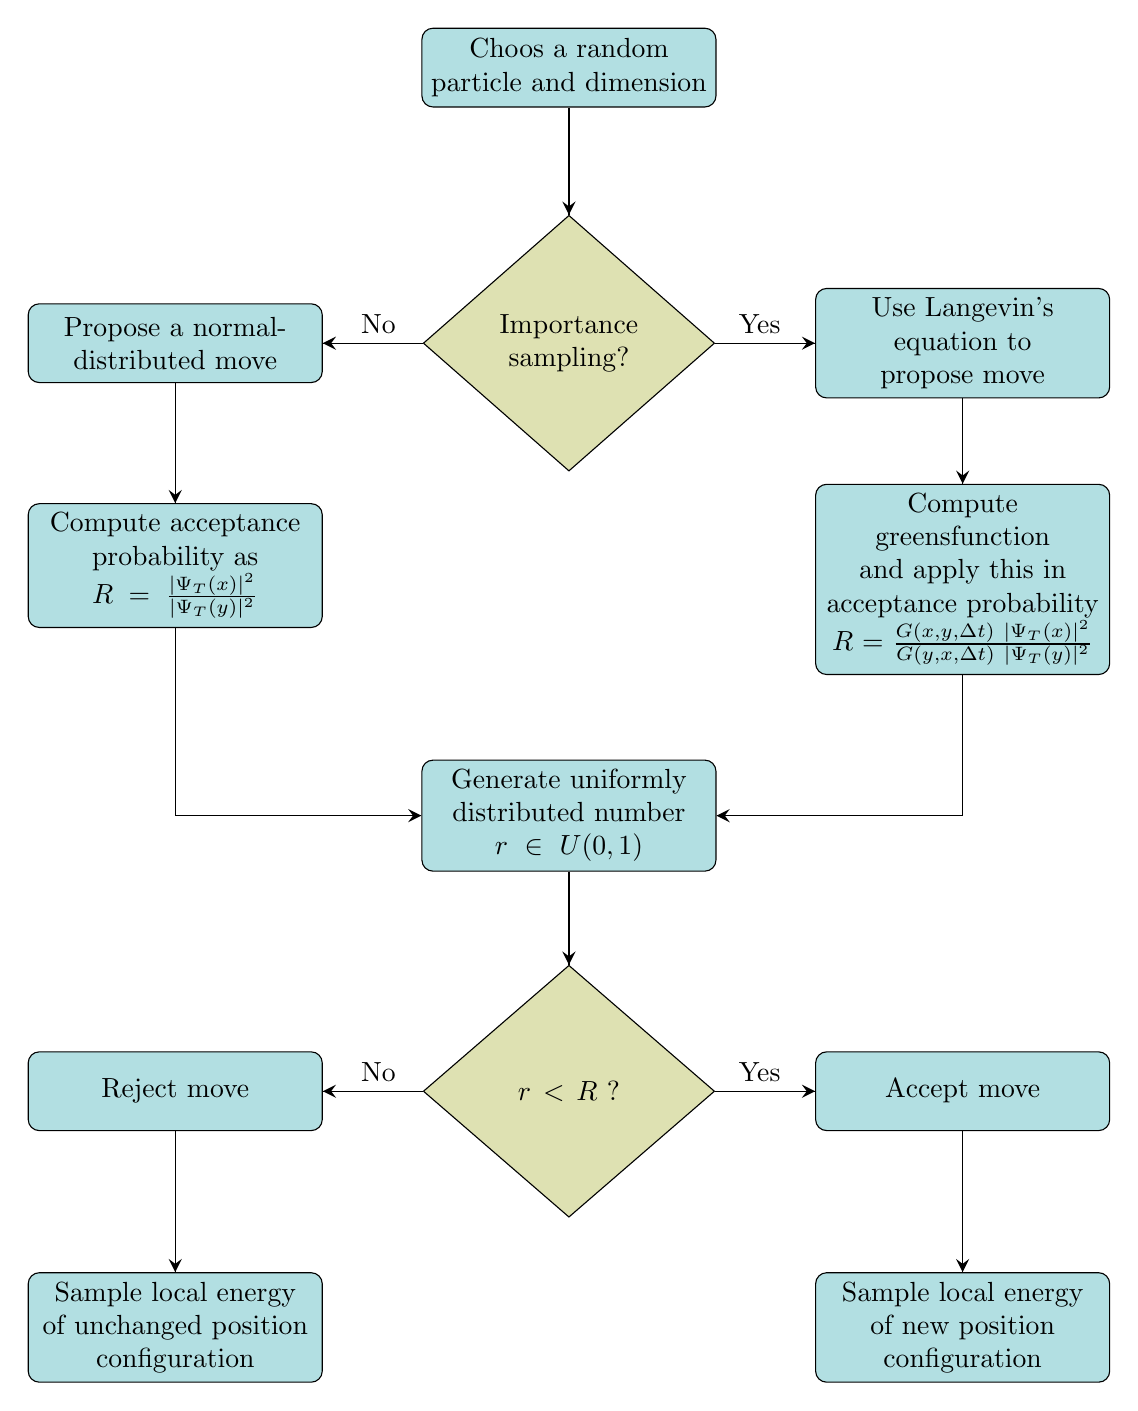
\begin{tikzpicture} [node distance=3cm]
			\node (particleAndDimension) [roundrect] {Choos a random particle and dimension};% of one particle in one dimension};
			
			\node (importance test)[decision, below of=particleAndDimension, yshift=-0.5cm]{Importance sampling?};
			
			\node (Langevin) [roundrect,right of=importance test, xshift=2cm] {Use Langevin's equation to propose move};
			\node (importance ratio) [roundrect,below of=Langevin] {
				Compute greensfunction and apply this in acceptance probability\\
				$R = \frac{G(x,y,\Delta t)~|\Psi_T(x)|^2}{G(y,x,\Delta t)~|\Psi_T(y)|^2}$};
			
			\node (unimportant move) [roundrect,left of=importance test, xshift=-2cm] {
				Propose a normal-distributed move};
			\node (standard ratio) [roundrect,below of=unimportant move, yshift=0.5em] {
				Compute acceptance probability as
				$R = \frac{|\Psi_T(x)|^2}{|\Psi_T(y)|^2}$};
			
			\node (random number)[roundrect, below of=importance test, yshift=-3.0cm]{
				Generate uniformly distributed number\\
				$r\in U(0,1)$	
			};
			\node (Accept)[decision, below of=random number, yshift=-0.5cm]{
				$r<R$~?
			};
			
			\node (Accepted) [roundrect,right of=Accept, xshift=2cm] {Accept move};
			\node (New sample)[roundrect,below of=Accepted]{Sample local energy of new position configuration};
			
			
			\node (Rejected) [roundrect,left of=Accept, xshift=-2cm] {Reject move};
			\node (Old sample)[roundrect,below of=Rejected]{Sample local energy of unchanged position configuration};
			
			
			
			\draw [arrow] (particleAndDimension) -- (importance test);
			\draw [arrow] (importance test) -- node [anchor=south, xshift=-0.2em]{Yes} (Langevin);
			\draw [arrow] (Langevin) --(importance ratio);
			\draw [arrow] (importance ratio) |- (random number) ;
			\draw [arrow] (importance test) -- node [anchor=south, xshift=0.2em]{No} (unimportant move);
			\draw [arrow] (unimportant move) -- (standard ratio);
			\draw [arrow] (standard ratio) |- (random number);
			\draw [arrow] (random number) -- (Accept);
			\draw [arrow] (Accept) -- node [anchor=south, xshift=-0.2em]{Yes} (Accepted);
			\draw [arrow] (Accept) -- node [anchor=south, xshift=0.2em]{No} (Rejected);
			\draw [arrow] (Accepted) -- (New sample);
			\draw [arrow] (Rejected) -- (Old sample);
			
			\end{tikzpicture}
		\end{center}
	\end{figure}
	
	
	
	\subsection{Optimizing parameters}
	Our trail wavefunctions, both for the two-body system \eqref{TwoBodyTrailWavefunction} and many-body system \eqref{ManyBodyWavefunction}, contain two variational parameters, $\alpha$ and $\beta$.
	In the VMC approach, the minimal energy is sought. Therefore, the goal is to minimize $\langle E_L\rangle$ with respect to these variational parameters.
	There are several ways to minimize a value with respect to some parameters, and here we will use the method of steepest descent (SD). The SD method, in algorithm form, is:
	
	\begin{equation}
		\vec{x}_{n+1} = \vec{x}_n - \gamma_n\nabla f
	\end{equation}
	where $\vec{x}$ is a vector containing the variables for which one wishes to find the minimum of $f$, $\gamma$ is a steplength and $n$ is an index expressing the number of iterations. In application to the current problem, $f = \langle E_L\rangle$, and $\vec{x}=\lr{\alpha, \beta}$. The above equation can thus be rewritten as
	\begin{equation}
	\lr{\alpha, \beta}_{n+1} = \lr{\alpha, \beta}_n - \gamma_n(\frac{\partial}{\partial \alpha}, \frac{\partial}{\partial \beta})  \langle E_L\rangle. \label{optimizationAlgo}
	\end{equation}
	
	 However, since $\langle E_L\rangle$ is an expensive quantity to find numerically, and its derivatives ($\bar{E}_\alpha \equiv \frac{d\langle E_L\rangle}{d\alpha}$ and $\bar{E}_\beta \equiv \frac{d\langle E_L\rangle}{d\beta}$) even more so, an analytical expression is desirable. This can be found as follows:
	
	\begin{align}
	\begin{split}
	\bar{E}_\alpha &= \frac{d}{d\alpha}\int dx P(x) E_L\\
	&= \frac{d}{d\alpha}\int dx \frac{|\psi|^2}{\int dx'|\psi|^2}\frac{1}{\psi}H\psi\\
	&= \frac{d}{d\alpha}\int dx \frac{\psi^*H\psi}{\int dx'|\psi|^2}
	\end{split}
	\end{align}
	
	Since the Hamiltonian is hermitian, one has $\int dx\psi^* H \psi = \int dx H\psi^*\psi$, giving:
	
	\begin{align}
	\begin{split}
	&= \frac{d}{d\alpha}\int dx \frac{H\psi^*\psi}{\int dx'|\psi|^2}\\
	&= \left[ \int dx\frac{H\left(\psi^*\left(\frac{d\psi}{d\alpha}\right) + \left(\frac{d\psi^*}{d\alpha}\right)\psi\right)}{\int dx'|\psi|^2} \right] - \left[ \int dx \frac{H\psi^*\psi}{\left(\int dx'|\psi|^2\right)^2}\int dx'\left( \psi^*\left(\frac{d\psi}{d\alpha}\right) + \left(\frac{d\psi^*}{d\alpha}\psi\right) \right) \right]
	\end{split}
	\end{align}
	
	Again one may use the hermiticity of the Hamiltonian to get $\int dx H \psi^*\left(\frac{d\psi}{d\alpha}\right) = \int dx H \left(\frac{d\psi^*}{d\alpha}\right)\psi$. So:
	
	\begin{align}
	\begin{split}
	&= 2\left[ \int dx\frac{H\psi^*\frac{d\psi}{d\alpha}}{\int dx'|\psi|^2} \right] - 2\left[ \int dx \frac{H\psi^*\psi}{\left(\int dx'|\psi|^2\right)^2}\int dx' \psi^*\frac{d\psi}{d\alpha} \right]\\
	&= 2\left[ \int dx\frac{H\psi^*\frac{d\psi}{d\alpha}}{\int dx'|\psi|^2} - \int dx \frac{H\psi^*\psi}{\int dx'|\psi|^2}\int dx' \frac{1}{\int dx'|\psi|^2}\psi^*\frac{d\psi}{d\alpha} \right]\\
	&= 2\left[ \int dx\frac{\psi^*\left(\frac{E_L}{\psi}\frac{d\psi}{d\alpha}\right) \psi}{\int dx'|\psi|^2} - \int dx \frac{\psi^* E_L\psi}{\int dx'|\psi|^2}\int dx' \frac{\psi^*\left(\frac{1}{\psi}\frac{d\psi}{d\alpha}\right)\psi}{\int dx'|\psi|^2} \right]\\
	&= 2\left( \langle\frac{\bar{\psi}_\alpha}{\psi}E_L\rangle -  \langle\frac{\bar{\psi}_\alpha}{\psi}\rangle\langle E_L\rangle \right)
	\end{split}
	\end{align}
	where $\bar{\psi}_\alpha \equiv \frac{d\psi}{d\alpha}$. Obviously, the derivative with respect to $\beta$ produce an equivalent result. 
	
	
	% ENDED HERE BRUH. WHY NOT PICK IT UP? 
	In order to find the optimal parameters, the once that give minimal energy, we set a criteria that if the new parameters, $\vec{x}_{n+1}$, suggested by equation \eqref{optimizationAlgo} has a shorter gradient than the current, $\vec{x}_n$, we accept this change, whereas if it doesn't we reset the parameters to the current and shorten the steplength by a factor 0.7. We are content when the length of the gradient is sufficiently short and store these values as the optimal parameters. 
	
	The optimal parameters produced is not trivial, though. As illustrated in figure \ref{fig:energyPlot15x15N2} the minimum value of the local energy is much more strongly dependent on the value of $\alpha$ than the value of $\beta$ in the two-electron system. Our approach will most likely produce a value of $\alpha$ that is in agreement with the true minimum, but our value of $\beta$ may differ somewhat. However, this difference does not seem to have much of a consequence for this system. For the case of the two-electron system the optimal paramaters produced were $\alpha=1.003$ and $\beta=0.3$, which resulted in a local energy of $\bk{E_L} = 3.003$. This is sufficiently close to the real minimum of 3, and seem to be in agreement with the figure as well.
	
	
	
\begin{figure}[H]
\centering
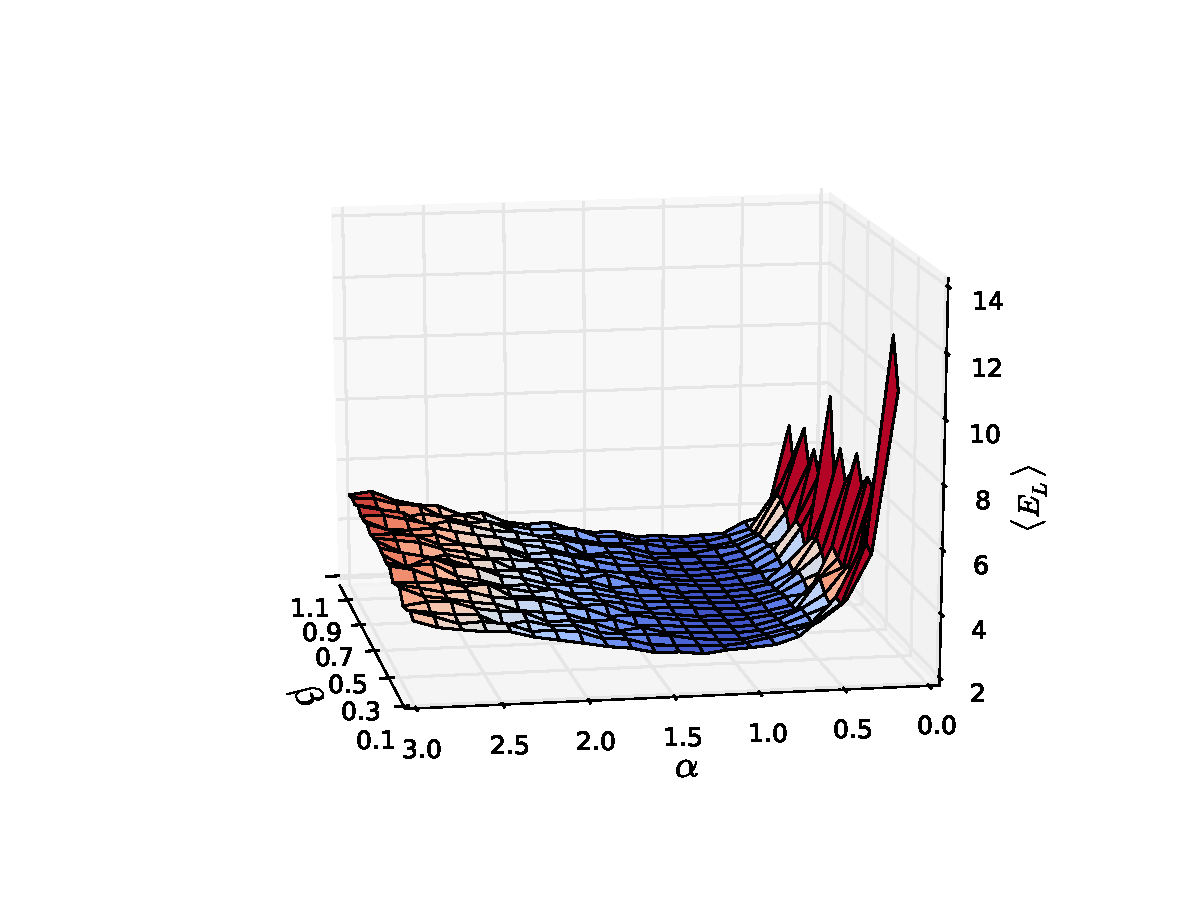
\includegraphics[width=0.8\linewidth, trim={0 2cm 0 4.5cm}, clip]{figures/energySurface/energyPlot15x15N2}
\caption{Local energy as a function of the parameters $\alpha$ and $\beta$ in the two-electron system.}
\label{fig:energyPlot15x15N2}
\end{figure}
	
	
	
	
		\begin{table}[H]
			\begin{center}
				\caption{Optimal parameters}
				\begin{tabularx}{\textwidth}{@{}YYYYY@{}}
					$N$	& $\omega$ & $\bk{E_L}$ & $\alpha$ & $\beta$\\
					\toprule
					2	&	1.00 & & & \\
						&	0.50 & & & \\
						&	0.10 & & & \\
						&	0.05 & & & \\
						&   0.01 & & & \\
					\midrule
					8   &	1.00 & & & \\
						&	0.50 & & & \\
						&	0.10 & & & \\
						&	0.05 & & & \\
						&   0.01 & & & \\
					\midrule
					12  &	1.00 & & & \\
						&	0.50 & & & \\
						&	0.10 & & & \\
						&	0.05 & & & \\
						&   0.01 & & & \\
					\midrule
					20  &	1.00 & & & \\
						&	0.50 & & & \\
						&	0.10 & & & \\
						&	0.05 & & & \\
						&   0.01 & & & \\
					\bottomrule
				\end{tabularx}
				\label{tab:Optimal parameters}
			\end{center}
		\end{table}
	
	
	
	
	
	
	
	
	
	
	
	
	
	\subsection{Benchmarking}
	While the flowchart seems nice and compact, there is quite a bit code that needs implementing and some benchmarks would be nice. The first is so check if the program reproduces the energy expected for non-interacting electrons in a harmonic oscillator potential. This means that if we remove the Coulomb potential and set $a_{ij} = 0$, we should get the energies shown in table \ref{tab:nonint_noJ_energies}. If these values are reproduced, it means our Slater determinant expressions are correctly implemented.
	
	
	\begin{table}[H]
		\begin{center}
			\caption{Harmonic oscillator energies}
			\begin{tabularx}{0.5\textwidth}{@{}YY@{}}
				N	&	E [$\omega$]\\
				\midrule
				2	&	2\\
				6	&	10\\
				12	&	28\\
				20	&	60
			\end{tabularx}
			\label{tab:nonint_noJ_energies}
		\end{center}
	\end{table}
	
	Another benchmark is to reproduce the results of our program for the two body quantum dot. This system was solved analytically, and thus would show that the many body program can reproduce analytical results for 2 particles. Obviously, this means that the full problem (Coulomb interactions and Jastrow correlations) works, at least for the two body system.\\
	
	
	
	\section{Results}
	
	Without any interaction in the system, no Coulomb potential or Jastrow factor, we are left with a simple harmonic oscillator with energies given as
	\begin{equation}
	E_{n_x,n_y} = \hbar\omega\lr{n_x + n_y +1}.
	\end{equation}
	
	
	\begin{figure}[H]
		\begin{center}
			\begin{tikzpicture}
			\begin{scope}[xshift=0cm, yshift = 0cm]
			\draw (0,0) -- (1,0);
			\draw [arrow] (0.33,-0.3)--(0.33,0.3);
			\draw [arrow] (0.66,0.3)--(0.66,-0.3);
			\end{scope}	
			
			\foreach \i in {-1,1}{
				\begin{scope}[xshift=\i cm, yshift = 1cm]
				\draw (0,0) -- (1,0);
				\draw [arrow] (0.33,-0.3)--(0.33,0.3);
				\draw [arrow] (0.66,0.3)--(0.66,-0.3);
				\end{scope}	
			}
			\foreach \i in {-2,0,2}{
				\begin{scope}[xshift=\i cm, yshift = 2cm]
				\draw (0,0) -- (1,0);
				\draw [arrow] (0.33,-0.3)--(0.33,0.3);
				\draw [arrow] (0.66,0.3)--(0.66,-0.3);
				\end{scope}	
			}
			\foreach \i in {-3,-1,1,3}{
				\begin{scope}[xshift=\i cm, yshift = 3cm]
				\draw (0,0) -- (1,0);
				\draw [arrow] (0.33,-0.3)--(0.33,0.3);
				\draw [arrow] (0.66,0.3)--(0.66,-0.3);
				\end{scope}	
			}
			
			\node [draw=none] (N2)  at (6.5,0) {$E_L = 2\phantom{0}$};
			\node [draw=none] (N6)  at (6.5,1) {$E_L = 10$};
			\node [draw=none] (N12) at (6.5,2) {$E_L = 28$};
			\node [draw=none] (N20) at (6.5,3) {$E_L = 60$};
			\draw [dotted, thick] (2,0) -- (N2);
			\draw [dotted, thick] (3,1) -- (N6);
			\draw [dotted, thick] (4,2) -- (N12);
			\draw [dotted, thick] (5,3) -- (N20);
			
			\end{tikzpicture}
		\end{center}
		\caption{Illustrative figure of spin configurations in the closed shell system.}
		\label{fig: spinFig}
	\end{figure}
	
	
	
	
	
	
	
	
	
	
	
	\begin{table}[H]
		\begin{center}
			\caption{Local energy computed for systems without the Jastrow factor and Coulomb potential. This resembles a pure harmonic oscillator and the results are dead on.}
			\begin{tabularx}{0.5\textwidth}{@{}YYY@{}}
				\toprule
				$N$& $E_L$& $\sigma$ \\*
				\midrule
				2  & 2  & 0 \\
				6  & 10 & 0 \\
				12 & 28 & 0 \\
				20 & 60 & 0 \\
				\bottomrule
			\end{tabularx}
			\label{tab:HO}
		\end{center}
	\end{table}
	These result infer that our Slater determinants are implemented correctly.
	
	
	
	\begin{table}[H]
		\begin{center}
			\caption{Expectation value of the kinetic energy and potential energy for several values of $\omega$.}
			\begin{tabularx}{0.5\textwidth}{@{}YYYY@{}}
				\toprule
				$\omega$& $\bk{E_K}$& $\bk{E_P}$ & $\bk{E_L}$ \\*
				\midrule
				0.01 & 0.0122 & 0.0969 & 0.0863\\
				0.05 & 0.0511 & 0.2274 & 0.2769\\
				0.1  & 0.0939 & 0.3544 & 0.4593\\
				1.0  & 0.8983 & 2.1475 & 3.0002\\
				\bottomrule
			\end{tabularx}
			\label{tab:varousOmega}
		\end{center}
	\end{table}
	
	Note, though, that each of the values listed in table \ref{tab:varousOmega} are from individual runs.
	The expectation values of the kinetic, potential and total (local) energy are thus not from the same simulation, and their value might not add up perfectly as $E_L = E_K + E_P$.
	The total energy is only shown to give a sense of its magnitude.
	
	
	For 
	
	
	
	
	
	
	
	\section{Comments}
	
	
\end{document}